\documentclass[12pt, letterpaper]{article}
\usepackage{lmodern}
\usepackage{graphicx}
\graphicspath{{images/}}
\usepackage{amsmath} % For the equation* environment

\title{My first LaTeX document}
\author{Bartek Pacia\thanks{Funded by the Overleaf team.}}
\date{November 2024}

\begin{document}

    % This is a sample doc comment

    \maketitle


    \section{Intro}\label{sec:intro}

    We have now added a title, author and date to our first \LaTeX{} document!

    First document.
    This is a simple example, with no extra parameters or packages included.

    Lorem ipsum dolor sit amet, consectetur adipiscing elit.
    Ut congue et velit non laoreet.
    Sed aliquet eros ut massa bibendum viverra.
    Nullam non imperdiet magna, eget condimentum ex.
    Praesent gravida consequat elit nec faucibus.
    Morbi vitae feugiat leo, at semper erat.`
    Vestibulum dapibus leo metus.
    Vivamus in ipsum sit amet eros vehicula imperdiet.
    Blah blah.

    Donec rhoncus tortor ac neque gravida condimentum.
    In cursus sodales laoreet.
    Duis eu interdum leo.
    Fusce ut varius ligula.
    Nulla commodo mollis vehicula.
    Ut tempus ante metus, ac elementum felis bibendum et.
    Aliquam eros mi, rutrum quis quam sed, pulvinar tristique felis.
    In malesuada massa et auctor tincidunt.
    Donec porttitor gravida erat, ac molestie erat ullamcorper eget.

    Some of the \textbf{greatest} discoveries in \underline{science} were made by \textbf{\textit{accident}}.

    Some of the greatest \emph{discoveries} in science were made by accident.

    \textit{Some of the greatest \emph{discoveries} in science were made by accident.}

    \textbf{Some of the greatest \emph{discoveries} in science were made by accident.}


    \section{Images}\label{sec:images}

    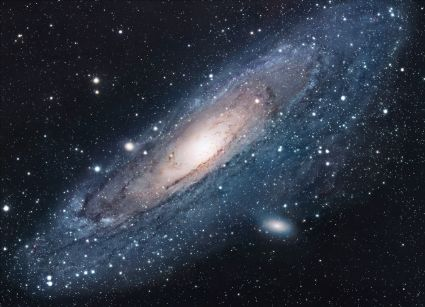
\includegraphics{universe}

    There's a picture of a galaxy above.

    \begin{figure}[h]
        \centering
        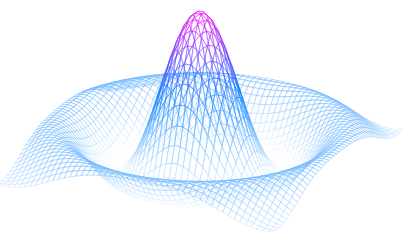
\includegraphics[width=0.75\textwidth]{mesh}
        \caption{A nice plot.}
        \label{fig:mesh1}
    \end{figure}

    As you can see in figure~\ref{fig:mesh1}, the function grows near the origin.
    This example is on page~\pageref{fig:mesh1}.


    \section{Creating lists}\label{sec:creating-lists}

    An unordered list:

    \begin{itemize}
        \item The individual entries are indicated with a black dot, a so-called bullet.
        \item The text in the entries may be of any length.
    \end{itemize}

    \noindent An ordered list:

    \begin{enumerate}
        \item This is the first entry in our list.
        \item The list numbers increase with each entry we add.
    \end{enumerate}


    \section{Math}\label{sec:math}

    In physics, the mass-energy equivalence is stated by the equation $E=mc^2$, discovered in 1905 by Albert Einstein.

    \begin{math}
        E=mc^2
    \end{math} is typeset in a paragraph using inline math mode---as is $E=mc^2$, and so too is \(E=mc^2\).

    The mass-energy equivalence is described by the famous equation\[ E=mc^2 \] discovered in 1905 by Albert Einstein.

    In natural units ($c = 1$), the formula expresses the identity
    \begin{equation}
        E=m
    \end{equation}

    Subscripts in math mode are written as $a_b$ and superscripts are written as $a^b$.
    These can be combined and nested to write expressions such as

    \[ T^{i_1 i_2 \dots i_p}_{j_1 j_2 \dots j_q} = T(x^{i_1},\dots,x^{i_p},e_{j_1},\dots,e_{j_q}) \]

    We write integrals using $\int$ and fractions using $\frac{a}{b}$.
    Limits are placed on integrals using superscripts and subscripts:

    \[ \int_0^1 \frac{dx}{e^x} =  \frac{e-1}{e} \]

    Lower case Greek letters are written as $\omega$ $\delta$ etc.
    while upper case Greek letters are written as $\Omega$ $\Delta$.

    Mathematical operators are prefixed with a backslash as $\sin(\beta)$, $\cos(\alpha)$, $\log(x)$ etc.

    \subsection{First example}\label{subsec:first-example}

    The well-known Pythagorean theorem \(x^2 + y^2 = z^2\) was proved to be invalid for other exponents, meaning the next equation has no integer solutions for \(n>2\):

    \[ x^n + y^n = z^n \]

    \subsection{Second example}\label{subsec:second-example}

    This is a simple math expression \(\sqrt{x^2+1}\) inside text.
    And this is also the same:
    \begin{math}
        \sqrt{x^2+1}
    \end{math}
    but by using another command.

    This is a simple math expression without numbering
    \[\sqrt{x^2+1}\]
    separated from text.

    This is also the same:
    \begin{displaymath}
        \sqrt{x^2+1}
    \end{displaymath}

    \ldots and this:
    \begin{equation*}
        \sqrt{x^2+1}
    \end{equation*}

\end{document}
